\subsection{RQ1: Representation and Model-Conditioned Gap}
\label{sec:ev-rq1}

RQ1 asks whether the capability model can represent what tools and models do well enough to decide what a
request needs. We test three of its ingredients: the typing $\tau$ on which structural reasoning relies, the
measured reliability profile $\rho_{\mathrm{LLM}}$ that decides which operations the model keeps, and the gap of
Algorithm~1 that turns the two into a toolkit.

\emph{Protocol.} Typing is scored against the blind labels $J_B$ (labelled evidence). The profile is measured on
a calibration suite of 432 generated data operations (extraction, classification, counting, approximate sums,
exact computation and joins; 10 to 640 records; English and French; clean or noisy text; isolated or embedded in a
multi-step context). Claude Haiku, Sonnet and Opus answered every item by reading only, without tools, and
stated beforehand, per cell, their probability of answering correctly. The threshold $\tau$ is chosen on 264
calibration items as the smallest value whose selective risk, the false-native rate among operations kept
native, is at most the risk target, and is evaluated on 168 held-out items (measured evidence). One Opus batch of
45 items was interrupted by a usage limit; its items are excluded for Opus, not counted as errors. The gap is
exercised on the review scenario of Fig.~1 for growing inputs.

\begin{figure}[t]
\centering
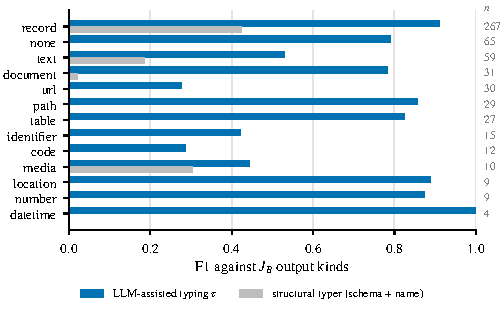
\includegraphics[width=\columnwidth]{fig_rq1_typing}
\caption{Typing agreement with $J_B$ per output kind (kinds with at least four tools; right: support). The
LLM-assisted typing $\tau$ is compared with a structural typer that uses schemas and names only.}
\label{fig:ev-typing}
\end{figure}

\emph{Typing.} The LLM-assisted typing agrees with $J_B$ on 78.9\% of output kinds ($\kappa=0.718$, macro-F1
0.704) but on only 35.7\% of complete types (kind and domain). A structural typer working from schemas and names
alone reaches 22.8\% ($\kappa=0.070$, macro-F1 0.062) and recognises only records, text, documents and media
at all (F1 at most 0.42; Fig.~\ref{fig:ev-typing}); $\tau$ itself is weakest on URLs, code and identifiers (F1
0.28--0.42). Types are therefore reliable at the
kind level and unreliable at the domain level, which is where structural matching discriminates; this limits
structural retrieval (Section~\ref{sec:ev-rq3}).

\begin{figure*}[t]
\centering
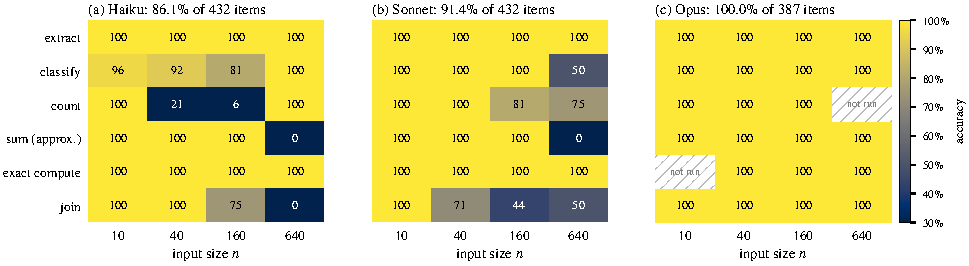
\includegraphics[width=\textwidth]{fig_rq1_calibration}
\caption{Measured reliability per operation and input size for three models (calibration suite, both splits;
cells average languages, noise and context). Hatched cells belong to the interrupted Opus batch.}
\label{fig:ev-calibration}
\end{figure*}

\begin{table}[t]
\centering
\caption{Model-profile calibration: accuracy (Wilson 95\% CI), self-assessment calibration, and the held-out
behaviour of the threshold $\tau$ chosen for a 5\% risk target (measured profile) versus the 64-item profile at
$\tau=0.9$. Cov.: share of operations kept native; FNR: false-native rate (errors among them).}
\label{tab:ev-calibration}
\scriptsize
\setlength{\tabcolsep}{2.2pt}
\begin{tabular}{@{}lrcrrrrrrrr@{}}
\toprule
 & & & & \multicolumn{2}{c}{Self-assess.} & \multicolumn{3}{c}{Measured, risk 5\%} & \multicolumn{2}{c}{64-item} \\
\cmidrule(lr){5-6}\cmidrule(lr){7-9}\cmidrule(l){10-11}
Model & $n$ & Accuracy (\%) & $n{=}640$ & ECE & Brier & $\tau$ & Cov. & FNR & Cov. & FNR \\
\midrule
Haiku & 432 & 86.1 [82.5, 89.1] & 67 & 0.39 & 0.30 & 0.21 & 83 & 3.6 & 21 & 0.0 \\
Sonnet & 432 & 91.4 [88.4, 93.7] & 62 & 0.20 & 0.11 & 0.42 & 90 & 3.3 & 26 & 4.5 \\
Opus & 387 & 100.0 [99.0, 100.0] & 100 & 0.38 & 0.20 & 0.90 & 100 & 0.0 & -- & -- \\
\bottomrule
\end{tabular}
\end{table}


\emph{Capability boundaries.} Table~\ref{tab:ev-calibration} and Fig.~\ref{fig:ev-calibration} show that the
boundary between native and tool-requiring operations depends on the model and on the operation, not only on
the input size. Haiku answers 86.1\% of the items (95\% CI 82.5--89.1\%) and fails counting already at medium
sizes (21\% at $n=40$, 6\% at $n=160$); Sonnet answers 91.4\% (88.4--93.7\%) and loses joins as they grow (71\%
at $n=40$, 44\% at $n=160$); both fail approximate sums over 640 numbers. Opus answers all 387 items it was given,
so its boundary lies beyond the suite. Language matters little (Haiku 88.0\% in English against 84.3\% in
French; Sonnet 91.2\% against 91.7\%), whereas noise lowers Sonnet from 95.4\% to 87.5\% and exactness lowers
Haiku from 92.5\% (tolerant) to 78.1\% (exact). A single profile per model family would thus misplace the boundary
in both directions.

\begin{figure*}[t]
\centering
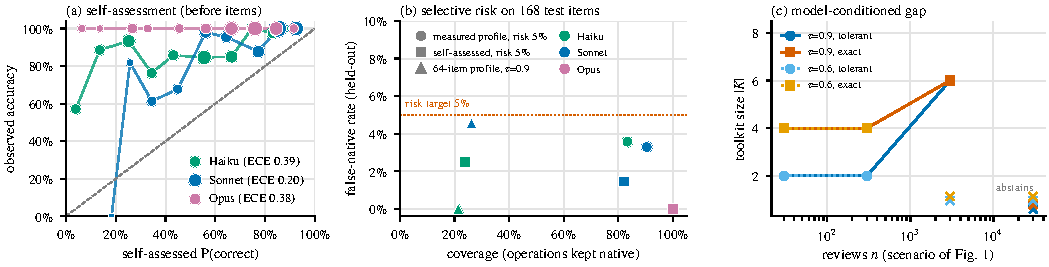
\includegraphics[width=\textwidth]{fig_rq1_profile}
\caption{(a) Reliability diagram of the models' self-assessment, given before any item was seen (marker area:
items per bin). (b) Held-out coverage and false-native rate of three profiles for each model. (c) Toolkit size
of the review scenario against the input size, Sonnet profile; crosses mark abstentions.}
\label{fig:ev-profile}
\end{figure*}

\emph{Measured against self-assessed reliability.} All three models underestimate themselves
(Fig.~\ref{fig:ev-profile}a): their stated probabilities average 0.47, 0.72 and 0.62 against accuracies of 0.86,
0.91 and 1.00 (ECE 0.39, 0.20 and 0.38). With the measured profile and a 5\% risk target, the held-out
false-native rate stays within the target for every model (3.6\%, 3.3\% and 0.0\%) while 83\%, 90\% and 100\% of
the operations remain native (Fig.~\ref{fig:ev-profile}b). The 64-item profile used before this revision is
safe but wasteful at $\tau=0.9$: it keeps only 21\% (Haiku) and 26\% (Sonnet) of the operations native and sends
most of the work the models perform correctly to tools. Self-assessment cannot replace measurement: at the same
target it keeps 24\% of Haiku's operations native. On the test and development tasks the measured profile
overrules 12 of the analyst's 128 claims that an operation is native (9.4\%).

\emph{Model-conditioned gap.} On the review scenario the gap behaves as designed (Fig.~\ref{fig:ev-profile}c):
with tolerant aggregation two tools suffice at $n=30$ and 300, where the model keeps 60\% of the goals, and six
are needed at $n=3{,}000$; exact aggregation adds two tools at the small sizes; at $n=30{,}000$, and at
$n=3{,}000$ with $\tau=0.6$, the engine abstains instead of returning an unsupported toolkit. Without gap
analysis it abstains in every setting, because no registry tool serves the scenario's interpretive goals.

\emph{Interpretation.} The representation supports model-conditioned discovery: what a request needs depends on
the deployed model, and a measured profile with a risk-targeted threshold bounds the false-native rate on held-out
operations at the chosen level. Two limits remain. The suite covers six data operations, not the whole
transformation vocabulary of Definition~6, and Opus reaches its ceiling; profile stability across model updates
was not measured. Typing is the weaker ingredient: its domain-level disagreement propagates to every structural
decision evaluated next.
